	\documentclass{article}
			
		\usepackage{parskip}
		\usepackage{listings}
		\usepackage{xcolor}
		\usepackage{textcomp}
			
		%STYLE AND COLOR DEFINITION FOR SOURCE CODE 	
		\newcommand{\PHPamountofcolor}{75}
		\newcommand{\SourceCodeContext}{5}
		%Lets define the php language colors:
		\definecolor{PHP_comment_old}{HTML}{FF8000}
		\colorlet{PHP_comment}{PHP_comment_old!\PHPamountofcolor!black}
		\definecolor{PHP_default_old}{HTML}{000000}
		\colorlet{PHP_default}{PHP_default_old!\PHPamountofcolor!black}
		\definecolor{PHP_keyword_old}{HTML}{6c9c11}
		\colorlet{PHP_keyword}{PHP_keyword_old!\PHPamountofcolor!black}
		\definecolor{PHP_emph1_old}{HTML}{0F58A2}
		\colorlet{PHP_emph1}{PHP_emph1_old!\PHPamountofcolor!black}
		\definecolor{PHP_emph2_old}{HTML}{CCAA00}
		\colorlet{PHP_emph2}{PHP_emph2_old!\PHPamountofcolor!black}
		\definecolor{PHP_emph4_old}{HTML}{C60484}
		\colorlet{PHP_emph4}{PHP_emph4_old!\PHPamountofcolor!black}
		\definecolor{PHP_string_old}{HTML}{C78F0A}
		\colorlet{PHP_string}{PHP_string_old!\PHPamountofcolor!black}
		\definecolor{PHP_variable_old}{HTML}{C82210}%C82210
		\colorlet{PHP_variable}{PHP_variable_old!\PHPamountofcolor!black}
		\definecolor{PHP_number_old}{HTML}{BF1CA6}
		\colorlet{PHP_number}{PHP_number_old!\PHPamountofcolor!black}
		%Now we want to highlight the variables. This will be done by triggering the function \PHPhighlightvar at the start of any $ run. This function wil only highlight variables and any other identifiers will be ignored. Luckily lstlisting will only give correct identifiers so we only will have to check if the previous call was made with a $
		\usepackage{fontspec}
		\setmonofont{Courier}
		%\usepackage[utf8]{inputenc}
		%\usepackage[T1]{fontenc}
		%\usepackage{courier, textcomp}
		\usepackage{etoolbox}
		\newtoggle{InString}{}% Keep track of if we are within a string
		\togglefalse{InString}% Assume not initally in string
		
		\newcommand*{\ColorIfNotInString}[1]{\iftoggle{InString}{#1}{\color{PHP_number}#1}}%

		%helper
		
		\newcommand{\PHPhighlightvar}[1]{\ifnum\theDollarFlag=1 \color{PHP_variable} \fi#1\setcounter{DollarFlag}{0}}
		\newcounter{DollarFlag}
		
		%images
		\usepackage{graphicx}
		\graphicspath{ {images/} }
		\usepackage{wrapfig}
		\usepackage{subcaption}
		
		
			
			
			
		
			
			\title{Machine Learning: Fourth Home Work \\ \bigskip \large Support Vector Machines}

			\author{Edoardo Ghini}
			
			\begin{document}
			
			\textbf{\maketitle}
			\pagenumbering{gobble}
			
			\bigskip\bigskip\bigskip
			\begin{center}
			
\includegraphics[width=0.5\textwidth]{laSapienza}
			\end{center}
			\bigskip\bigskip\bigskip
			\textbf{
			Dipartimento di Ingegneria dell'Università di Roma La Sapienza}
			

			\newpage
			\pagenumbering{roman}
			\tableofcontents
			\newpage
			\pagenumbering{arabic}
			
			
			
			
			
			%SETTING STYLE OF SOURCE CODE
			\lstset{
		  language        = php,
		  basicstyle      = \footnotesize\ttfamily,
		  keywordstyle    = \color{PHP_keyword},
		  stringstyle     = \color{PHP_string!90!black}\toggletrue{InString},
		  %this allows highlighting of variables:
		  literate        =  {\$}{{\iftoggle{InString}{\$}{\setcounter{DollarFlag}{1}\color{PHP_variable}\$\color{PHP_default}}}}1
		%    {"}{{{\ProcessQuote{"}}}}1% Disable coloring within double quotes
		%    {'}{{{\ProcessQuote{'}}}}1% Disable coloring within single quote
		    {0}{{{\ColorIfNotInString{0}}}}1
		    {1}{{{\ColorIfNotInString{1}}}}1
		    {2}{{{\ColorIfNotInString{2}}}}1
		    {3}{{{\ColorIfNotInString{3}}}}1
		    {4}{{{\ColorIfNotInString{4}}}}1
		    {5}{{{\ColorIfNotInString{5}}}}1
		    {6}{{{\ColorIfNotInString{6}}}}1
		    {7}{{{\ColorIfNotInString{7}}}}1
		    {8}{{{\ColorIfNotInString{8}}}}1
		    {9}{{{\ColorIfNotInString{9}}}}1,
		  identifierstyle = \color{PHP_default}\PHPhighlightvar,
		  commentstyle    = \color{PHP_comment}\slshape,
		  emph            =[1]{require_once, require, include_once, include, namespace, use, class, function, new},
		  emphstyle       =[1]\color{PHP_emph1},%\bf,
		  emph            =[2]{echo, empty, isset, array, instanceof},
		  emphstyle       =[2]\color{PHP_emph2},%\bf,
		  emph            =[3]{var, const, abstract, 
		                        protected, private, public,
		                        static, final, extends, implements,
		                        global, if, else, foreach ,for,
		                        endforeach, endif, endfor, elseif,
		                        as},
		  emphstyle       =[3]\color{PHP_keyword},%\bf,
		  emph            =[4]{return, throw, exit, __halt_compiler, continue, break},
		  emphstyle       =[4]\color{PHP_emph4},%\bf,
		  breaklines      = true,
		  captionpos      = b,
		  rulecolor       =\color{black},
		  keywords    ={__halt_compiler,    abstract,   and,    array,
		                    as, break,  callable,   case,   catch,  class,
		                    clone,  const,  continue,   declare,    default,
		                    die,    do, echo,   else,   elseif,
		                    empty,  enddeclare, endfor, endforeach, endif,
		                    endswitch,  endwhile,   eval,   exit,   extends,
		                    final,  finally,    for,    foreach,    function,
		                    global, goto, if,   implements, include,
		                    include_once,   instanceof, insteadof,
		                    interface,  isset, list,    namespace,
		                    new,    or, print, private, protected,  public,
		                    require,    require_once, return,   static,
		                    switch, throw,  trait, try, unset, use, var,
		                    while,  xor,    yield,
		  },
		  numbers=left,
		  stepnumber=1,  
		  numberfirstline=true,
		  numberstyle=\footnotesize,
		  xleftmargin=4.0ex,
		  upquote=true,
		  showlines=true
		  }	
			
			\renewcommand{\lstlistingname}{Code}

			
			\part{Introduction}
			
				\section{Scope}
This time the aim of the assignment has been to comprehend the concept behind the classification through Support Vector Machines
				\section{Objectives}
				
				For the purpose of understanding SVM algorithm and theory, it will be executed a classification task with, at first, a linear SVM, and then with a non-linear one in order to proof that non-linearity brings better scores because of more flexible classification boundaries. At the end I will have to validate and test the performances of the classifier with a K-fold approach.

\newpage
			\part{Development}
				\section{Data Manipulations}
	At the beginning, after that the first two vectors of a dataset had been loaded, I obtained a separation in train, validation and test data.	
	
	

				\section{Linear SVM}
				\subsection{Theory pills}
				As shown in these figures, I have started with a lineal model that, being a SVM classifier, maximises the distance between the first points of two different classes and the decision linear function.
				This maximum problem tries to find the greatest area in the data space that can be considered neutral between two data point concentrations. There is also a coefficient ( C ) that allows a different weighting of the penalty for missclassification.
				
								\begin{center}
				\begin{figure}
\centering
        \begin{subfigure}[b]{0.48\textwidth}
                \centering
                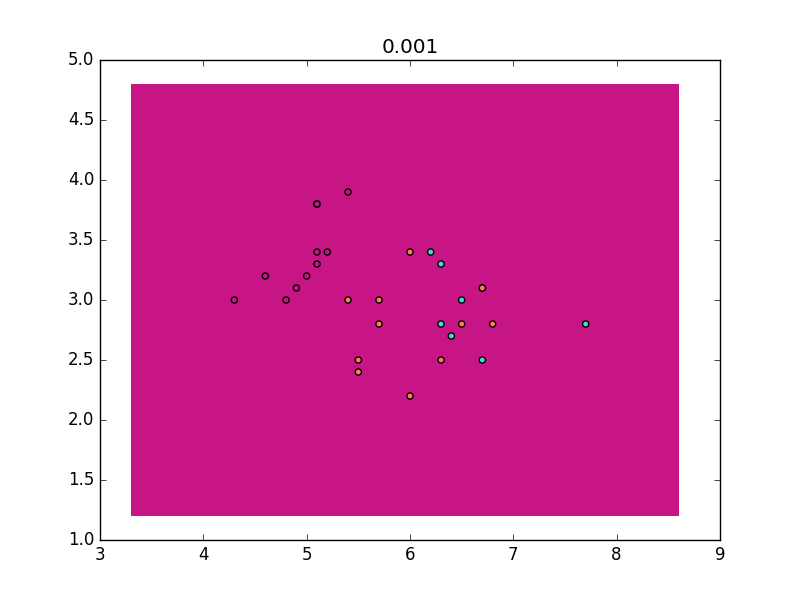
\includegraphics[width=\linewidth]{figure_1}
        \end{subfigure}\hfill
        \begin{subfigure}[b]{0.48\textwidth}
                \centering
                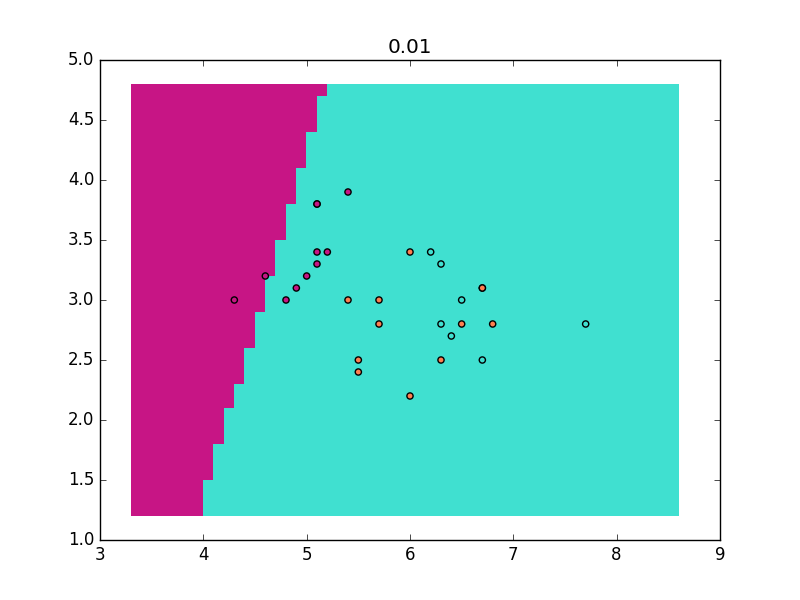
\includegraphics[width=\linewidth]{figure_2}
        \end{subfigure}\hfill
 \label{fig:1}
 \end{figure}
       
\begin{figure}
\centering  
        \begin{subfigure}[b]{0.48\textwidth}
                \centering
                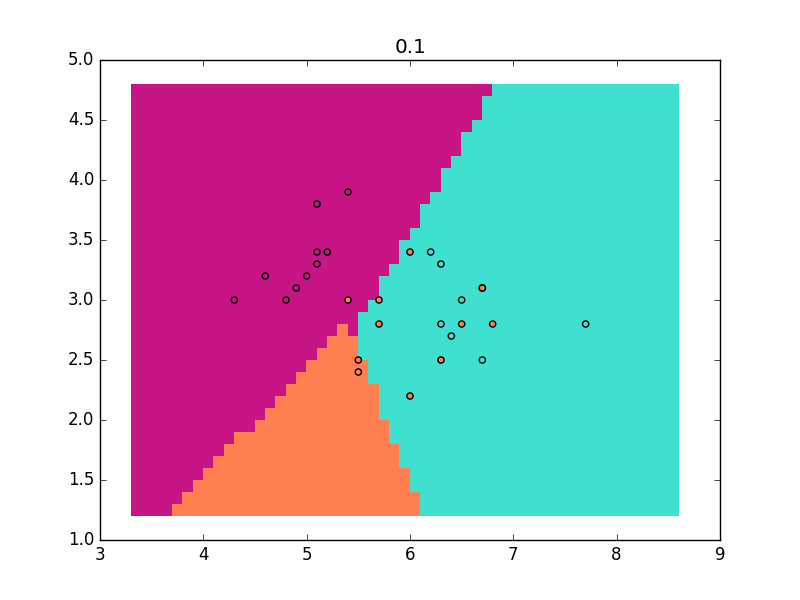
\includegraphics[width=\linewidth]{figure_3}
        \end{subfigure}\hfill
        \begin{subfigure}[b]{0.48\textwidth}
                \centering
                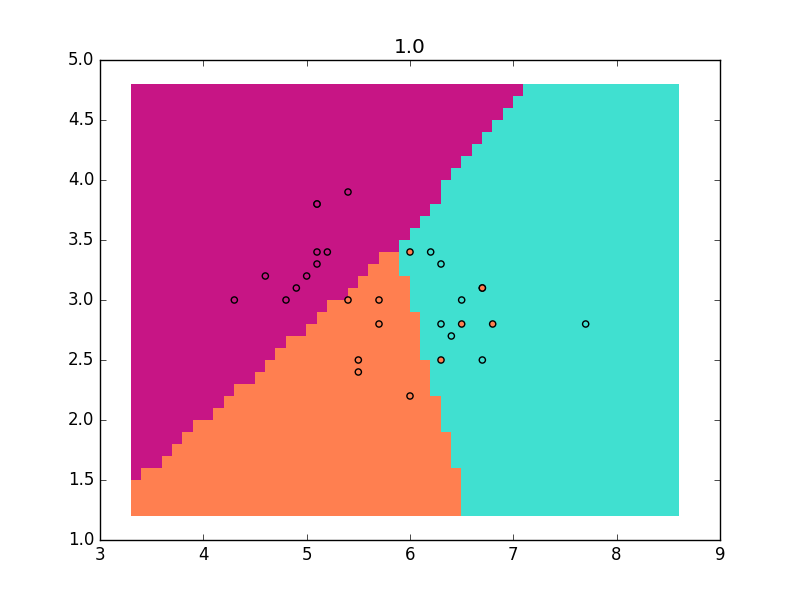
\includegraphics[width=\linewidth]{figure_4}
        \end{subfigure}
        \label{fig:2}
\end{figure}

\begin{figure}
\centering
        \begin{subfigure}[b]{0.48\textwidth}
                \centering
                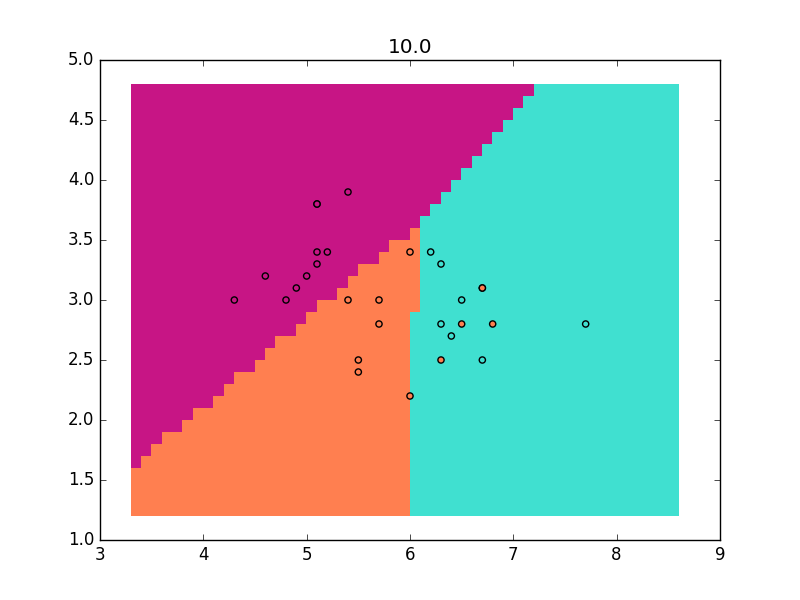
\includegraphics[width=\linewidth]{figure_5}
        \end{subfigure}\hfill
        \begin{subfigure}[b]{0.48\textwidth}
                \centering
                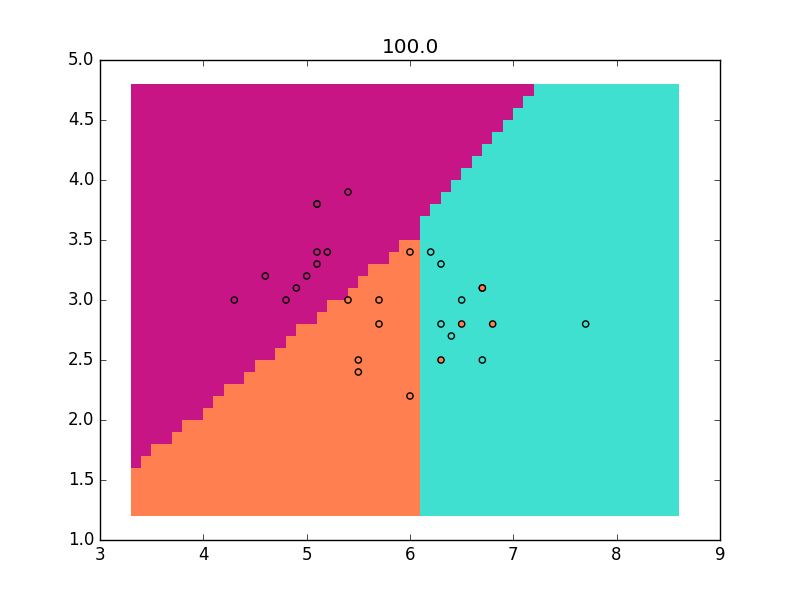
\includegraphics[width=\linewidth]{figure_6}
        \end{subfigure}\hfill
        \label{fig:3}
 \end{figure}
       
\begin{figure}
\centering
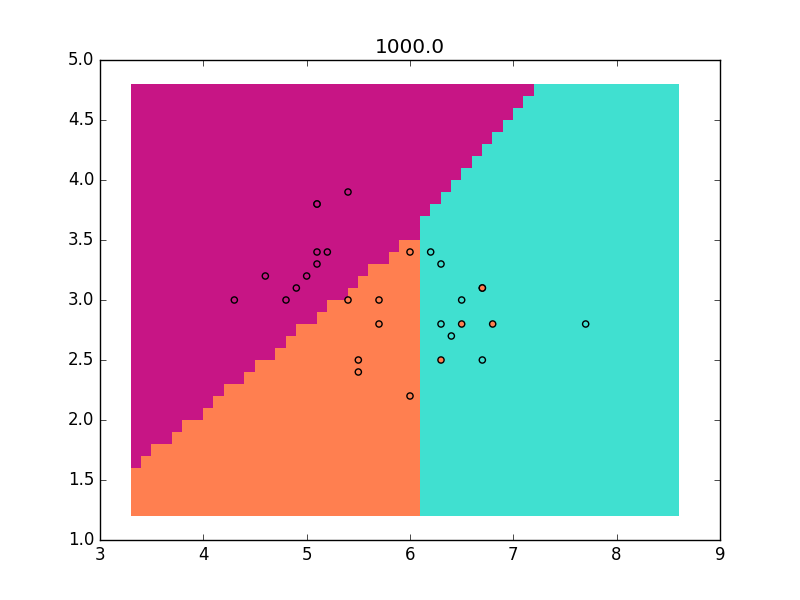
\includegraphics[width=0.9\textwidth]{figure_7}
\caption{}
\label{fig:4}
\end{figure}
\end{center}

\subsection{Validation and Test phases}
				The aforementioned figures have been generated with different values of C.
				In fig(5), it can be seen that for this dataset the best performances on the validation sets where obtained with a C parameters equal to 100.
\begin{center}
\begin{figure}
\centering
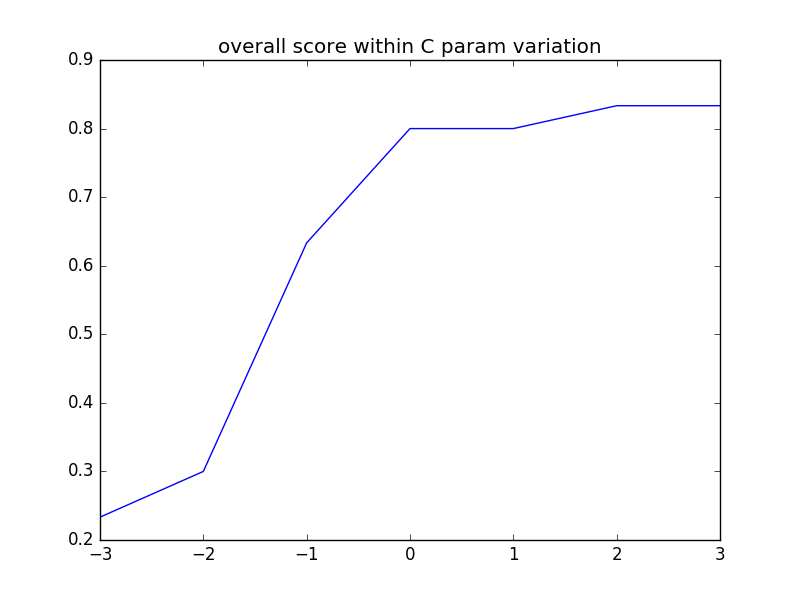
\includegraphics[width=0.9\textwidth]{figure_8}
\caption{}
\label{fig:5}
\end{figure}
\end{center}
				Correspondingly, in fig(6), we can see how this model performs on test data.
\begin{center}
\begin{figure}
\centering
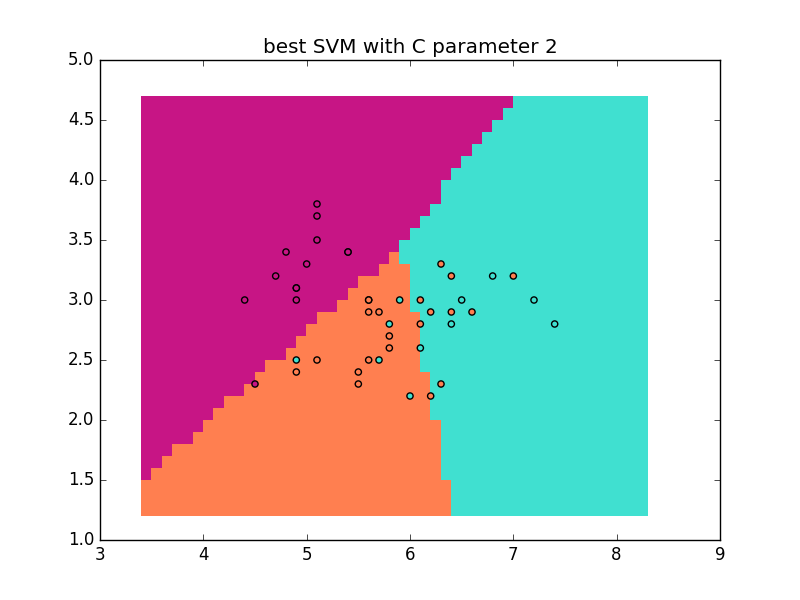
\includegraphics[width=0.9\textwidth]{figure_9}
\caption{}
\label{fig:6}
\end{figure}
\end{center}
\newpage
				
\section{Non-linear SVM}
\subsection{Training with C and gamma}
	Similarly, I repeated the same procedure with a Radial Basis Function Kernel. In practice, the model can decide smoother boundaries for data classification because of the kernel operation applied on the data in order to bring non-linearity.
	These figures are the results of a RBF SVM on the dataset with different values for C parameter. 
				
												\begin{center}
				\begin{figure}
\centering
        \begin{subfigure}[b]{0.48\textwidth}
                \centering
                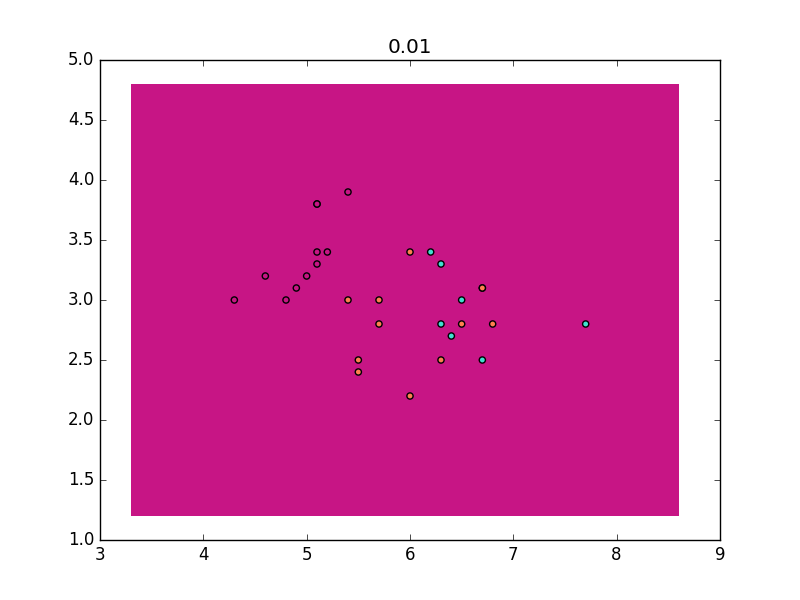
\includegraphics[width=\linewidth]{figure_11}
        \end{subfigure}\hfill
        \begin{subfigure}[b]{0.48\textwidth}
                \centering
                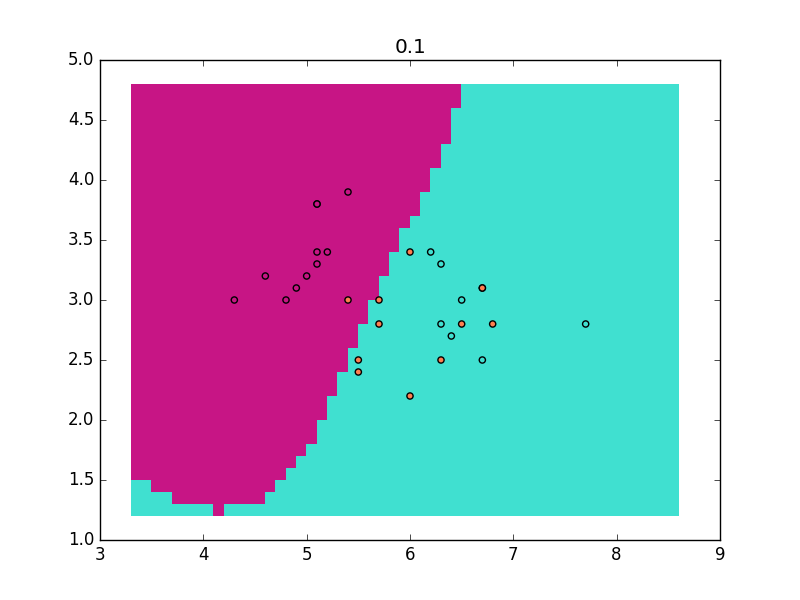
\includegraphics[width=\linewidth]{figure_12}
        \end{subfigure}\hfill
 \label{fig:7}
 \end{figure}
       
\begin{figure}
\centering  
        \begin{subfigure}[b]{0.48\textwidth}
                \centering
                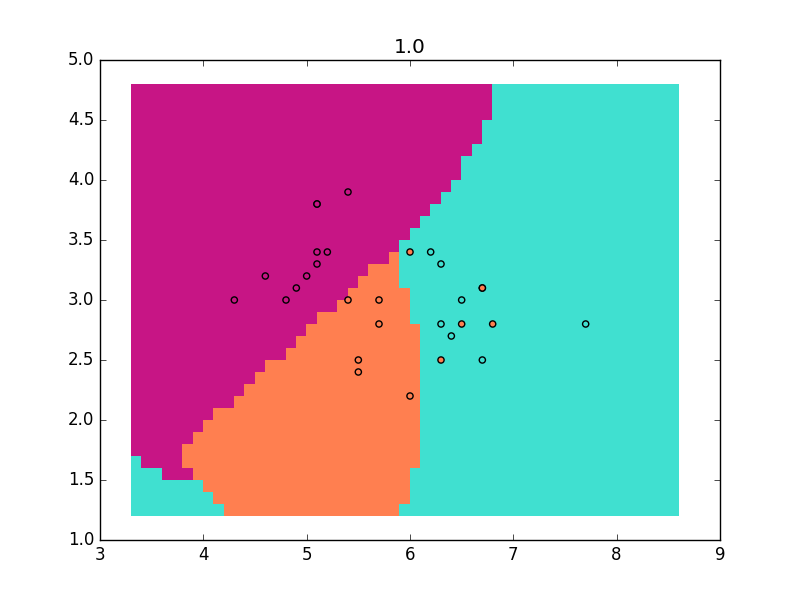
\includegraphics[width=\linewidth]{figure_13}
        \end{subfigure}\hfill
        \begin{subfigure}[b]{0.48\textwidth}
                \centering
                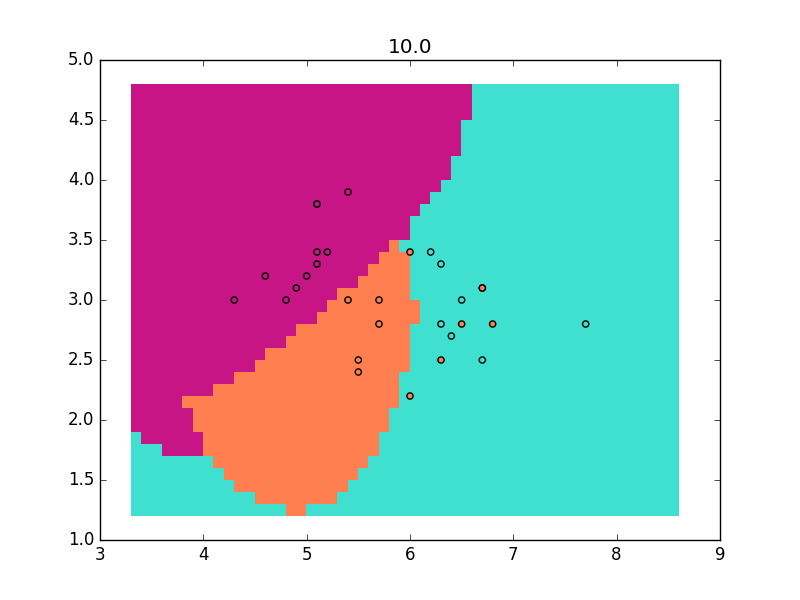
\includegraphics[width=\linewidth]{figure_14}
        \end{subfigure}
        \label{fig:8}
\end{figure}

\begin{figure}
\centering
        \begin{subfigure}[b]{0.48\textwidth}
                \centering
                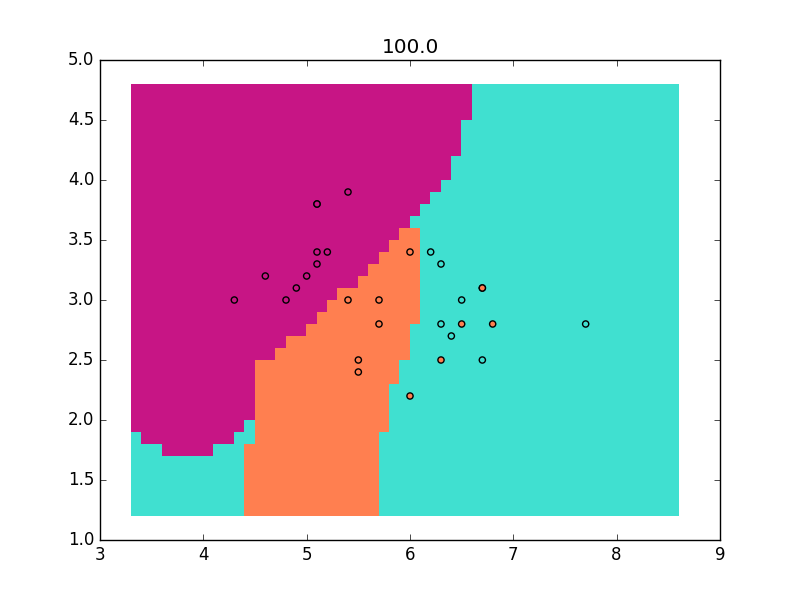
\includegraphics[width=\linewidth]{figure_15}
        \end{subfigure}\hfill
        \begin{subfigure}[b]{0.48\textwidth}
                \centering
                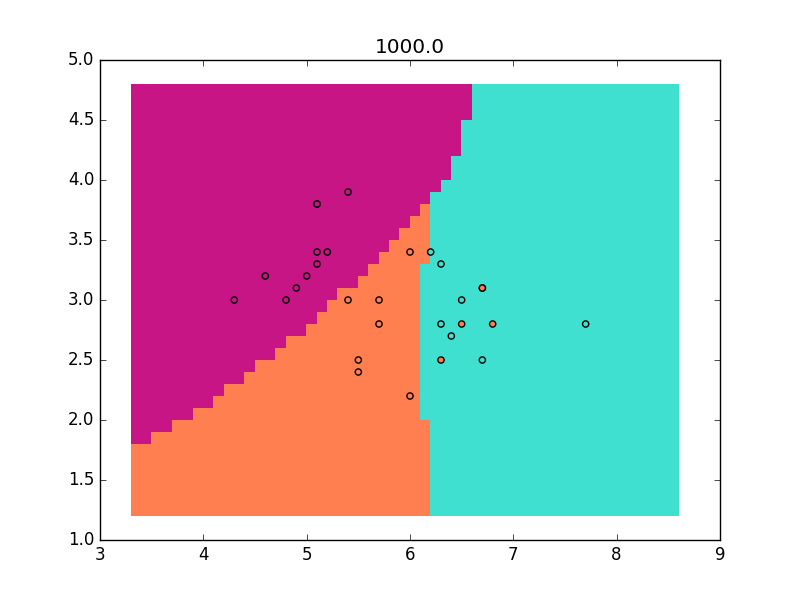
\includegraphics[width=\linewidth]{figure_16}
        \end{subfigure}\hfill
        \label{fig:9}
 \end{figure}
\end{center}
\subsection{First scores}
				As shown in fig(10) the model, identically to the linear experiment, behaves better. with high values of C. In particular, in fig(11) there is the plot of the SVM that has performed better on validation dataset.
				\begin{center}
\begin{figure}
\centering
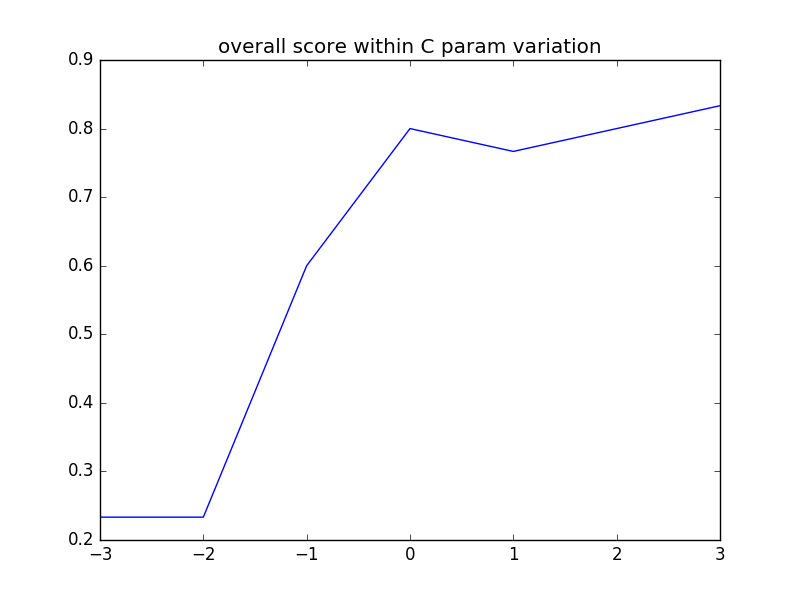
\includegraphics[width=0.9\textwidth]{figure_17}
\caption{}
\label{fig:10}
\end{figure}
\end{center}

				\begin{center}
\begin{figure}
\centering
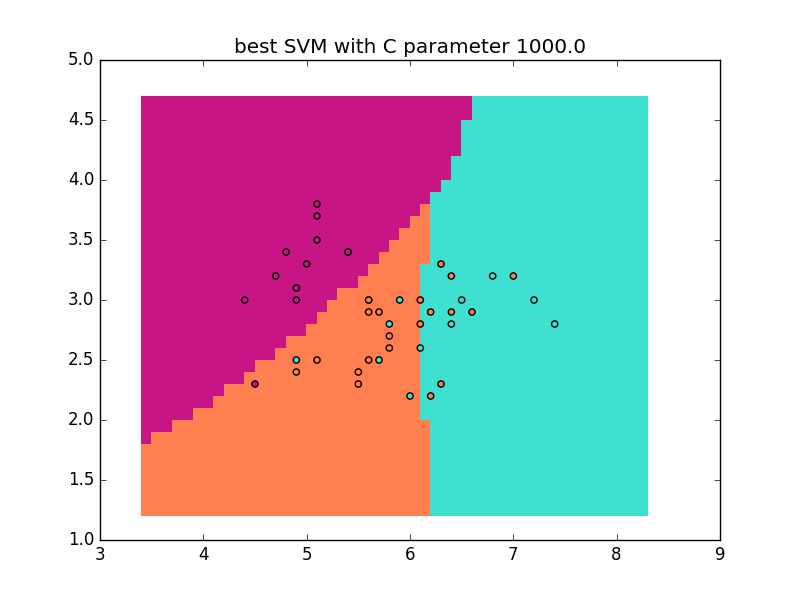
\includegraphics[width=0.9\textwidth]{figure_18}
\caption{}
\label{fig:11}
\end{figure}
\end{center}

\newpage

\subsection{Grid search with K-fold validation}
In order to chose the best classifier parameters, as shown in \ref{kfold} I merged together train and validation datasets and I set up an iterator that will be used to perform a k-fold validation.
 Subsequently, I managed to build up a grid search to find the best parameter combination of C and gamma.
 							\begin{lstlisting}[caption= Kfold wihin a grid search, label=kfold]
X_train_merged, X_test_merged, y_train_merged, y_test_merged= train_test_split(X, y,  test_size=split_rate_merged, random_state=20)

C_range = np.logspace(-3, 6, 10)
gamma_range = np.logspace(-6, 3, 10)
param_grid = dict(gamma=gamma_range, C=C_range)
cv = StratifiedShuffleSplit(n_splits=5, test_size=0.2, random_state=42)
grid = GridSearchCV(SVC(), param_grid=param_grid, cv=cv)
grid.fit(X_train_merged, y_train_merged)
\end{lstlisting}


 Gamma parameter seems to modify the way in which the classifier consider the significance of a data point according to his distance from the classification separator.
				
								\begin{center}

	
\newpage
			\part{Conclusions}
				
To sum up, in fig(12) is shown how a smart choice of parameters, in the case of a RBF classifier, C and gamma, could improve the score quality of the model.\medskip\\
This particular model with C =100 and gamma = 1 has performed a score of 0.86 on the validation set and of 0.68 on the merged set with further reliability due to the 5-fold validation.
\begin{figure}
\centering
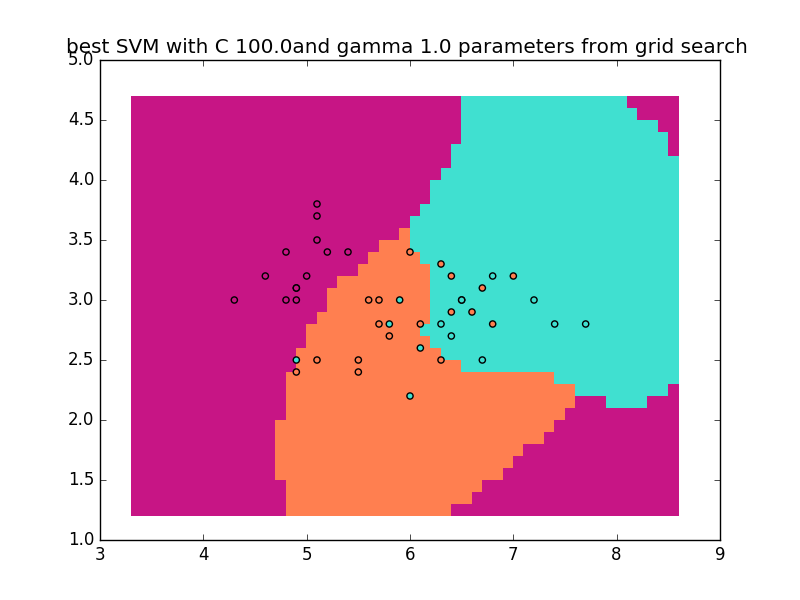
\includegraphics[width=0.9\textwidth]{figure_19}
\caption{}
\label{fig:12}
\end{figure}
\end{center}
			
		\end{document}
